\documentclass[11pt]{article}
\usepackage{graphicx}
\graphicspath{ {./images/} }

\usepackage{algorithm}
\usepackage{algpseudocode}
\usepackage{hyperref}

\usepackage{sectsty}
\usepackage{graphicx}
\usepackage[font=small,labelfont=bf]{caption} % Required for specifying captions to tables and figures

% Margins
\topmargin=-0.45in
\evensidemargin=0in
\oddsidemargin=0in
\textwidth=6.5in
\textheight=9.0in
\headsep=0.25in

\title{ %

\includegraphics[width=0.4\textwidth]{UniCT-Logo-Nero}~\\
A solution for MWVC using Iterated Local Search \\ 
\large Laboratorio Intelligenza Artificiale (LM-18) \\ Università degli Studi di Catania - A.A 2021/2022 \\
}
\author{ Danilo Leocata \\ Docente: Mario Pavone}
\date{\today}

\begin{document}

\maketitle	
\pagebreak

% Optional TOC
% \tableofcontents
% \pagebreak

%--Paper--

\section{Introduzione}

Si propone una soluzione per il Weight Vertex Cover problem utilizzando l'Iterated Local Search: l'obbiettivo proposto è trovare la migliore soluzione, data un istanza, con il minimo numero di iterazioni. Il codice è disponibile al \href{https://github.com/khalld/mwvc-using-ils-java}{seguente} repository di GitHub. \\
Il codice è stato implementato in Java utilizzando metodi custom. Inizialmente l'algoritmo è stato implementato con Python ma per via degli oneri computazionali (LPI richiedeva diverse ore per essere completato) è stato trovato più opportuno realizzare una versione in Java.
Prima di procedere con l'implementazione e la scelta dell'algoritmo, sono state consultate e prese in considerazioni varie pubblicazioni riguardanti la soluzione del problema (indicate a fine relazione). È stata trovata sin da subito interessante implementare una soluzione utilizzando l'Iterated Local Search, in particolare se ne propone una versione che perserva soluzioni non ottime sfruttando un \textit{term memory}.
Sfruttando l'ILS, è possibile ottenere sin da subito una soluzione \textit{completa} (intesa quando l'insieme dei nodi selezionati permette di raggiungere tutti i nodi dell'istanza) dopo poche iterazioni e migliorarla. Inoltre, sfruttando il \textit{term-memory} è possibile tenere traccia delle migliori soluzioni trovate permettendo di accettare e continuare la ricerca su soluzioni peggiori senza perderne traccia avendo la possibilità di ripescarle nell'operatore di perturbazione.

\pagebreak


\section{Validità della soluzione}

La soluzione è da considerarsi completa e valida se tutti gli archi del grafo sono esplorati. Di conseguenza è necessario controllare la validità della soluzione dopo la rimozione di un nodo.
È stato implementato un modo per effettuare il controllo di validità in maniera efficiente dimezzando il costo computazionale considerando uguali archi invertiti (\verb|(a,b) = (b,a))| come uguali.
È stata implementata una funzione per completare eventuali soluzioni non complete dalla \texttt{Perturbazione}.


\begin{algorithm}
    \caption{\texttt{CompleteSolution}}
    \begin{algorithmic}
        \Require {\texttt{perturbed solution}}
        
    
        \If{
            \State{\texttt{perturbed solution is complete}}
        }
            \State{\texttt{do nothing, return perturbed solution}}
        
        \Else{}
            \State{
                \While{
                    \State{\texttt{perturbed solution is complete}}
                }
                    \State{\texttt{
                        Get list of unselected nodes
                    }}
                    \State{\texttt{
                        find the best candidate node based on the number of knots (higher) or weight (lower) randomly and add to solution
                    }}
                \EndWhile

            }
        
        \EndIf{}
    \Return { \texttt{CompletePerturbedSolution}}
    \end{algorithmic}
    \end{algorithm}

Dai test effettuati è emerso che l'utilizzo dopo l'operatore di perturbazione tende a far bloccare la soluzione in un ottimo locale, di conseguenza verrà applicata solo dopo l'utilizzo della LocalSearch.

\section{ILS}

Sono stati testati sulle istanze due tipi di approcci:

\begin{itemize}
\item{costruzione di una soluzione a partire da un nodo iniziale scelto randomicamente;}
\item {scoperta della soluzione migliore partendo dalla soluzione peggiore (intesa così quella che ha selezionati tutti i nodi presenti nell'istanza);}
\end{itemize}

I diversi approcci producono circa gli stessi risultati. È stato preso in considerazione, ma scartato durante la fase di test, il random restart della soluzione dato che non ha portato migliorie al risultato finale.
Nel dettaglio, l'algoritmo ILS presentato parte dalla soluzione \textit{peggiore}, con tutti i nodi dell'istanza selezionati, e per mezzo dell'operatore di perturbazione e della local search si cercherà di ottimizzare la soluzione, oppure da una soluzione completa costruita
randomicamente 

\begin{algorithm}
\caption{\texttt{Iterated Local Search}}
\begin{algorithmic}
    \Require {\texttt{list of all nodes of instances}}

\State {\texttt{CurrentSolution = Solution with all available nodes selected or Randomly while is complete}}
\State {\texttt{initialize an empty term-memory}}
\While{ \texttt{max evaluations} }   

    \State {\texttt{SolutionToChange = CurrentSolution} }
    \State {\texttt{apply Perturbation to SolutionToChange} }
    \State {\texttt{apply LocalSearch to SolutionToChange} }
    \State{
        \If{\texttt{cost of SolutionToChange < cost of CurrentSolution and SolutionToChange not in term-memory}}
        \State {\texttt{add SolutionToChange in term-memory}}
        \EndIf
    }
    \State {\texttt{CurrentSolution = SelectCriteria(CurrentSolution, SolutionToChange, term-memory)}}
\EndWhile
\Return { \texttt{CurrentSolution}}
\end{algorithmic}
\end{algorithm}

\pagebreak

\section{Operatore di perturbazione}

L'idea generale della perturbazione è quella di modificare i parametri ad ogni iterazione applicando una perturbazione sui nodi selezionati dalla soluzione.
Un buon algoritmo deve evitare di far cadere sempre nello stesso minimo locale, in generale:

\begin{algorithm}
\caption{Perturbation}
\begin{algorithmic}
\Require{ \texttt{Solution} }
\State{\texttt{add random node from list of unselected if is possible}}
\State{\texttt{remove random node from list of already selected}}
\State{\Return{\texttt{solution}}}
\end{algorithmic}
\end{algorithm}

Sono state implementate due versioni di perturbazione rispettivamente: \verb|StrongPerturbation| che rimuove o aggiunge
randomicamente nodi da 1 o al massimo \verb|selectedNodes \ 2| e \verb|WeakPerturbation| che rimuove/aggiunge un solo nodo dalla soluzione.
Dai test effettuati portano circa agli stessi risultati. Inoltre è stato già dimostrato, da una delle referenze citate, che una perturbazione troppo forta porta allo stallo dell'ottimo locale.


Inoltre, tra le migliorie che la perturbazione potrebbe apportare alla soluzione vi è:
\begin{itemize}
\item{l'eliminazione automaticamente di cicli se questa contiene dei nodi ridondanti;}
\item{potrebbe rendere la soluzione non completa: di conseguenza applicando nuovamente la LocalSearch è possibile trovare un nodo candidato migliore rispetto a quello rimosso.}
\end{itemize}

\pagebreak

\section{Local Search e criterio di selezione del nodo migliore}

\begin{algorithm}
\caption{LocalSearch}
\begin{algorithmic}
\Require{ \texttt{Solution}}

\If{
    given solution has unreached nodes
}   
    \State\texttt{evaluate if swapping some nodes brings benefits to the solution }
    \State\texttt{increment counter for every evalutation}
\Else{}
\State\texttt{evaluate if removing some nodes brings benefits to the solution }
    \State\texttt{increment counter for every evalutation}
\EndIf{}

\State{\texttt{update solution}}

\State \Return updated solution
\end{algorithmic}
\end{algorithm}

\pagebreak

\section{Criterio di accettazione}

L'utilizzo del term memory permette di 'accettare' soluzioni peggiori rispetto ad altre e continuare la ricerca senza perder traccia di tutte le soluzioni trovate.
In sintesi, se la soluzione perturbata è simile alla corrente il criterio di accettazione può ripescare, randomicamente una delle soluzioni presenti nel \verb|term-memory| e continuare la ricerca.
È stato introdotto inolte un \verb|lockCounter| per evitare che la soluzione rimanga bloccata su un ottimo locale.


\begin{algorithm}
\caption{\texttt{Acceptance criteria}}
\begin{algorithmic}
    \Require \texttt{prev solution, new solution, term memory, lockCounter}
    \If{
        \State\texttt{cost old solution > cost new solution }
        \Return\texttt{new solution}
    }
    \Else{
        \State\texttt{if lockCounter = to maxValue}
        \State\Return\texttt{random solution from term-memory}
    }

    \EndIf{}
    
    \State \Return \texttt{random choice between (perturbed solution, current solution)}
\end{algorithmic}
\end{algorithm}

Tuttavia nella pratica questa ricerca non ha sempre portato a buoni risultati, di conseguenza è stato disabilitato.

\pagebreak

\section{Benchmarks e conclusione}

È stato implementato uno script che permette di salvare i benchmark le soluzioni ottenute dalle istanze su  file \verb|.csv|, oltre alla creazione dei grafici di convergenza.
I grafici importati ed le tabelle fanno riferimento alle run con \verb|WeakPerturbation|. n certi casi, si rimane bloccati su un ottimo locale per molto tempo, fino a quando una soluzione perturbata non ottimale fa da punto di partenza per trovare una soluzione migliore.
Si nota inoltre che un numero maggiore di nodi o archi non implica necessariamente un numero maggiore di valutazioni: anche grafi con lo stesso numero di nodi e archi hanno valori molto contrastanti, probabilmente perché il problema dipende molto dal peso dei nodi e dalla topologia del grafo.

\begin{center}
\begin{minipage}{0.48\linewidth}
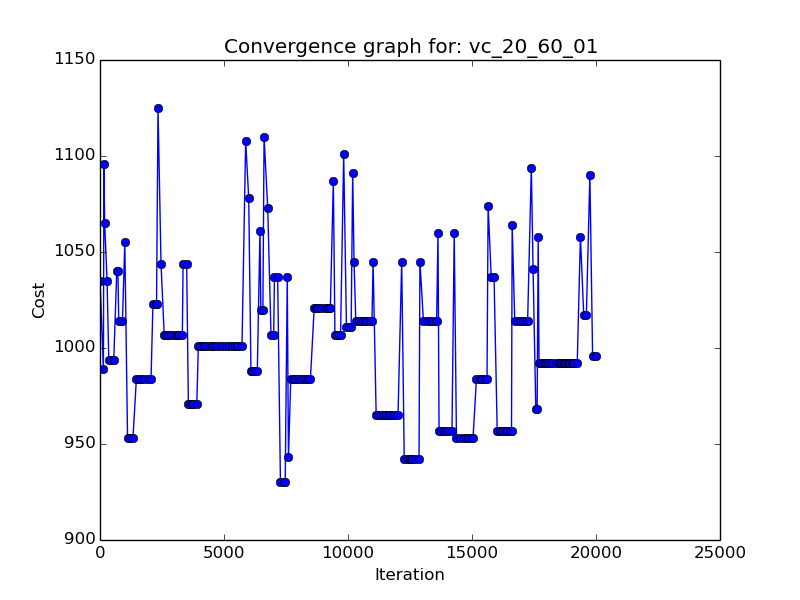
\includegraphics[width=\linewidth]{cg_1.png}
\end{minipage}%
\begin{minipage}{0.49\linewidth}
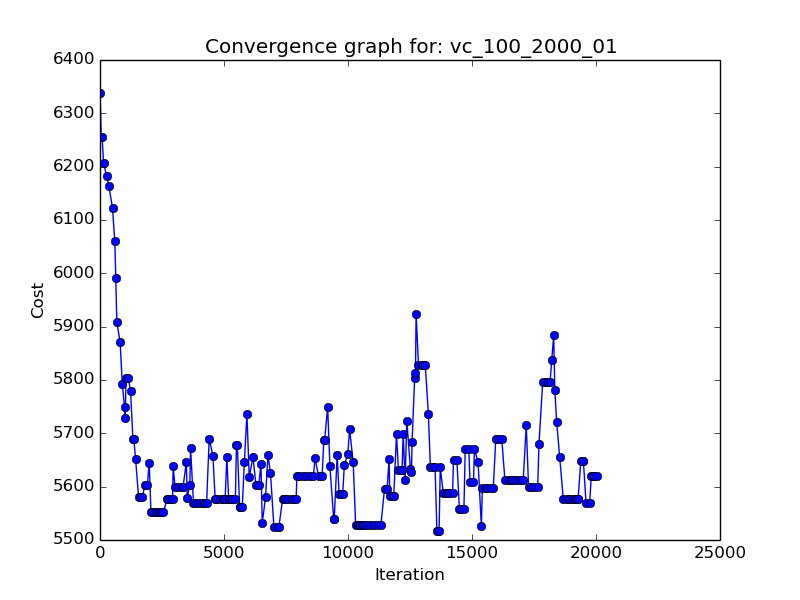
\includegraphics[width=\linewidth]{cg_2.png}
\end{minipage}
\begin{minipage}{0.49\linewidth}
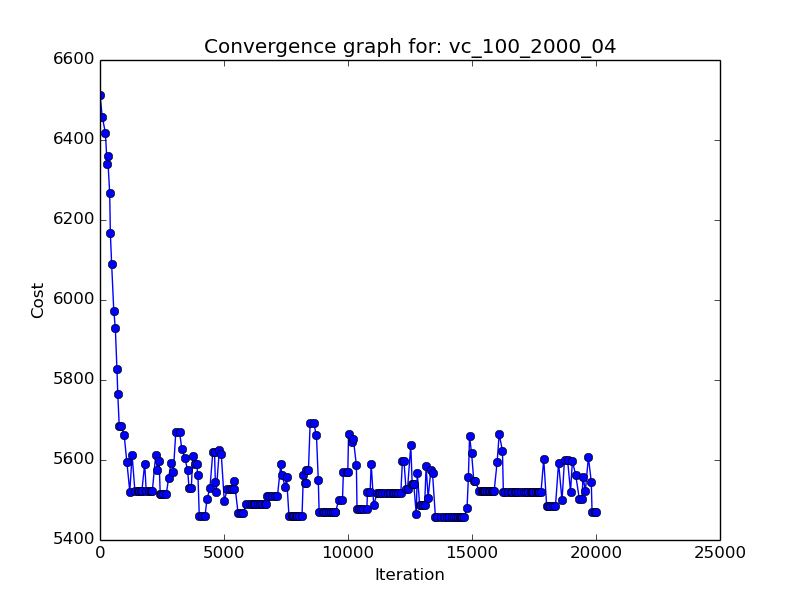
\includegraphics[width=\linewidth]{cg_3.png}
\end{minipage}
\begin{minipage}{0.49\linewidth}
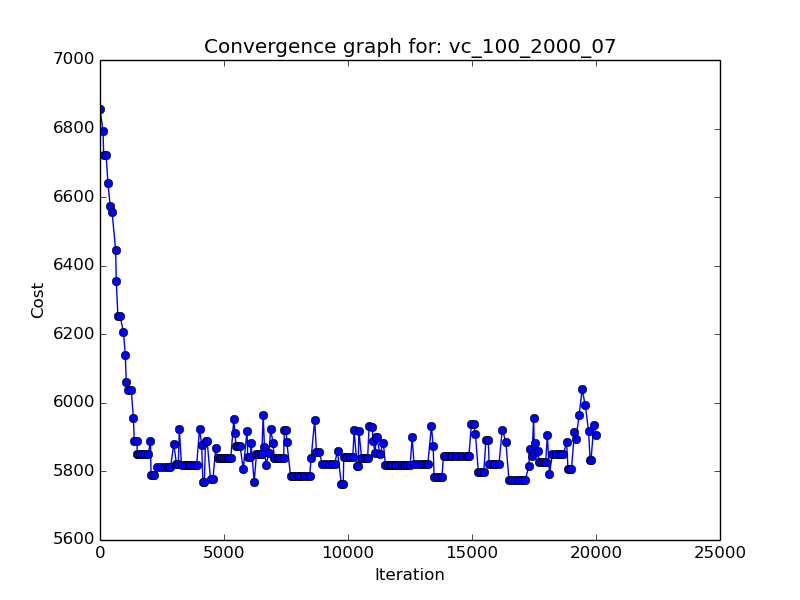
\includegraphics[width=\linewidth]{cg_4.png}
\end{minipage}
\captionof{figure}{Sample grafici di convergenza}
\end{center}

\pagebreak

\begin{table}[!ht]
    \centering
    \begin{tabular}{|l|l|l|l|}
    \hline
        instance & best solution & best solution iter & elapsed ms \\ \hline

        vc\_20\_120\_01 & 1253 & 77 & 99 \\ \hline
        vc\_20\_120\_02 & 1348 & 191 & 94 \\ \hline
        vc\_20\_120\_03 & 1319 & 58 & 92 \\ \hline
        vc\_20\_120\_04 & 1414 & 1179 & 99 \\ \hline
        vc\_20\_120\_05 & 1293 & 761 & 92 \\ \hline
        vc\_20\_120\_06 & 1271 & 77 & 102 \\ \hline
        vc\_20\_120\_07 & 1265 & 1806 & 98 \\ \hline
        vc\_20\_120\_08 & 1520 & 1654 & 98 \\ \hline
        vc\_20\_120\_09 & 1587 & 229 & 97 \\ \hline
        vc\_20\_120\_10 & 1452 & 381 & 95 \\ \hline
        vc\_20\_60\_01 & 1105 & 405 & 33 \\ \hline
        vc\_20\_60\_02 & 1585 & 476 & 37 \\ \hline
        vc\_20\_60\_03 & 1313 & 58 & 34 \\ \hline
        vc\_20\_60\_04 & 1177 & 115 & 37 \\ \hline
        vc\_20\_60\_05 & 1352 & 324 & 37 \\ \hline
        vc\_20\_60\_06 & 1426 & 343 & 33 \\ \hline
        vc\_20\_60\_07 & 1573 & 210 & 36 \\ \hline
        vc\_20\_60\_08 & 1526 & 39 & 36 \\ \hline
        vc\_20\_60\_09 & 1595 & 324 & 36 \\ \hline
        vc\_20\_60\_10 & 1416 & 552 & 35 \\ \hline
        vc\_25\_150\_01 & 1785 & 265 & 108 \\ \hline
        vc\_25\_150\_02 & 1472 & 241 & 103 \\ \hline
        vc\_25\_150\_03 & 1658 & 20000 & 105 \\ \hline
        vc\_25\_150\_04 & 1923 & 97 & 103 \\ \hline
        vc\_25\_150\_05 & 1792 & 1849 & 114 \\ \hline
        vc\_25\_150\_06 & 1651 & 505 & 99 \\ \hline
        vc\_25\_150\_07 & 1977 & 841 & 104 \\ \hline
        vc\_25\_150\_08 & 1693 & 361 & 107 \\ \hline
        vc\_25\_150\_09 & 1739 & 841 & 111 \\ \hline
        vc\_25\_150\_10 & 1547 & 553 & 102 \\ \hline
        vc\_200\_750\_01 & 14160 & 1991 & 280 \\ \hline
        vc\_200\_750\_02 & 13384 & 399 & 201 \\ \hline
        vc\_200\_750\_03 & 14509 & 6767 & 297 \\ \hline
        vc\_200\_750\_04 & 13230 & 797 & 306 \\ \hline
        vc\_200\_750\_05 & 14495 & 399 & 211 \\ \hline
        vc\_200\_750\_06 & 13586 & 1792 & 325 \\ \hline
        vc\_200\_750\_07 & 13197 & 7762 & 286 \\ \hline
        vc\_200\_750\_08 & 13676 & 9155 & 298 \\ \hline
        vc\_200\_750\_09 & 13710 & 200 & 208 \\ \hline
        vc\_200\_750\_10 & 13794 & 399 & 211 \\ \hline
    \end{tabular}
\end{table}

\pagebreak

\begin{table}[!ht]
    \centering
    \begin{tabular}{|l|l|l|l|}
    \hline
        instance & best solution & best solution iter & elapsed ms \\ \hline

        
        vc\_100\_2000\_01 & 7027 & 1189 & 3158 \\ \hline
        vc\_100\_2000\_02 & 6853 & 20000 & 2970 \\ \hline
        vc\_100\_2000\_03 & 6680 & 20000 & 3032 \\ \hline
        vc\_100\_2000\_04 & 6890 & 6535 & 2984 \\ \hline
        vc\_100\_2000\_05 & 7236 & 8812 & 3093 \\ \hline
        vc\_100\_2000\_06 & 6876 & 2080 & 2873 \\ \hline
        vc\_100\_2000\_07 & 7322 & 4753 & 3103 \\ \hline
        vc\_100\_2000\_08 & 7163 & 1090 & 2930 \\ \hline
        vc\_100\_2000\_09 & 6829 & 793 & 3073 \\ \hline
        vc\_100\_2000\_10 & 7238 & 1882 & 2977 \\ \hline
        vc\_100\_500\_01 & 6739 & 5446 & 252 \\ \hline
        vc\_100\_500\_02 & 7205 & 496 & 225 \\ \hline
        vc\_100\_500\_03 & 6764 & 10331 & 220 \\ \hline
        vc\_100\_500\_04 & 6818 & 9802 & 242 \\ \hline
        vc\_100\_500\_05 & 7185 & 2278 & 254 \\ \hline
        vc\_100\_500\_06 & 7228 & 3961 & 237 \\ \hline
        vc\_100\_500\_07 & 6763 & 194 & 81 \\ \hline
        vc\_100\_500\_08 & 6788 & 397 & 250 \\ \hline
        vc\_100\_500\_09 & 6894 & 193 & 226 \\ \hline
        vc\_100\_500\_10 & 6670 & 2773 & 244 \\ \hline
        vc\_200\_3000\_01 & 13795 & 200 & 2648 \\ \hline
        vc\_200\_3000\_02 & 13790 & 20000 & 4038 \\ \hline
        vc\_200\_3000\_03 & 14245 & 8956 & 4144 \\ \hline
        vc\_200\_3000\_04 & 15082 & 598 & 2681 \\ \hline
        vc\_200\_3000\_05 & 14095 & 9354 & 4136 \\ \hline
        vc\_200\_3000\_06 & 13731 & 2588 & 4196 \\ \hline
        vc\_200\_3000\_07 & 14247 & 16717 & 4083 \\ \hline
        vc\_200\_3000\_08 & 14197 & 200 & 3903 \\ \hline
        vc\_200\_3000\_09 & 14294 & 19901 & 4141 \\ \hline
        vc\_200\_3000\_10 & 13907 & 4976 & 3982 \\ \hline
        vc\_800\_10000 & 56404 & 6393 & 52037 \\ \hline

    \end{tabular}
\end{table}

\pagebreak

Una delle difficoltà più grandi trovate durante l'implementazione è stato quello di determinare se i criteri di scelta fossero effettivamente robusti o no. Sarebbe interessante proseguire con lo studio del problema continuando sui seguenti punti:

\begin{itemize}
    \item{implementare altri criteri per la selezione del nodo;}
    \item{implementare altri criteri di accettazione;}
    \item{perfezionare l'algoritmo su istanze piccole;}
    \item{minimizzare il numero di valutazioni della fitness;}
\end{itemize}

\pagebreak

\begin{thebibliography}{6}

\bibitem{1} \href{https://www.researchgate.net/publication/242463011_An_Effective_Algorithm_for_Minimum_Weighted_Vertex_Cover_problem}{An Effective Algorithm for Minimum Weighted Vertex Cover Problem}
\bibitem{2} \href{https://www.cs.umd.edu/class/fall2018/cmsc858E/pdfs/651/vc.pdf} {Two approximation algorithm for Vertex Cover} 
\bibitem{3} \href{https://ieeexplore.ieee.org/abstract/document/7550782}{A fast heuristic for the minimum weight vertex cover problem}
\bibitem{4} \href{https://www.researchgate.net/publication/242463011_An_Effective_Algorithm_for_Minimum_Weighted_Vertex_Cover_problem}{An Effective Algorithm for Minimum Weighted Vertex Cover Problem}
\bibitem{5} \href{https://www.sciencedirect.com/science/article/abs/pii/S0377221720300278}{A memory-based iterated local search algorithm for the multi-depot open vehicle routing problem}
\bibitem{6} \href{https://ieeexplore.ieee.org/document/7550782}{A fast euristic for the minimum weight vertex cover problem}

\end{thebibliography}


\pagebreak
%--/Paper--

\end{document}
